\documentclass[leqno,onefignum,onetabnum]{siamltex1213}
\usepackage{color}
\usepackage{xcolor}
\usepackage{url}
%\usepackage{ulem}
%\usepackage{mdwlist}
\usepackage{booktabs}
\usepackage{vuduc-stdpkgs}
\usepackage{vuduc-typography}
%\usepackage{placeins}
\usepackage{lscape}
\usepackage{amsmath}
\usepackage{amsfonts}
\usepackage{morefloats}
\setcounter{page}{1}
\pagenumbering{arabic}

\makeatletter
\newcommand{\ccell}[3][]{%
  \kern-\fboxsep
  \if\relax\detokenize{#1}\relax
    \expandafter\@firstoftwo
  \else
    \expandafter\@secondoftwo
  \fi
  {\colorbox{#2}}%
  {\colorbox[#1]{#2}}%
  {#3}\kern-\fboxsep
}
\makeatother
\definecolor{cellgray}{gray}{0.9}

\newcommand{\yesy}{\ccell{gray}{Y}}
\newcommand{\non}{N}
\newcommand{\myhline}{}
\newcommand{\TensorToolbox}{{\scshape Tensor Toolbox}\xspace}
\newcommand{\Cyclops}{{\scshape Cyclops}\xspace}
\newcommand{\MakeAcronym}[3]{
  \acrodef{#2}[{\scshape #2}]{#3}
  \newcommand{#1}{\ac{#2}\xspace}
}
\MakeAcronym{\CTF}{Ctf}{\Cyclops Tensor Framework}
\MakeAcronym{\BLAS}{Blas}{Basic Linear Algebra Subprograms}
\MakeAcronym{\BLIS}{Blis}{\BLAS-like Library Instantiation Software}
\MakeAcronym{\TTM}{Ttm}{tensor-times-matrix multiply}
\MakeAcronym{\InTTM}{InTtm}{in-place tensor-times-matrix multiply}
\MakeAcronym{\GEMM}{Gemm}{general matrix-matrix multiply}
\newcommand{\TMM}{\TTM} % synonym
% Additional math notation
\newcommand{\varTh}[1]{\ensuremath{{#1}^{\tiny\mbox{th}}}\xspace}
\newcommand{\T}[1]{\ensuremath{\mathbf{\underline{\uppercase{#1}}}}\xspace} % tensor
\newcommand{\M}[1]{\ensuremath{\mathbf{\uppercase{#1}}}\xspace} % matrix
\newcommand{\V}[1]{\ensuremath{\mathbf{\lowercase{#1}}}\xspace} % vector
\newcommand{\Msup}[2]{\ensuremath{\M{#1}^{^{(#2)}}}\xspace} % {matrix}^{(superscript)}
\newcommand{\Msub}[2]{\ensuremath{\M{#1}_{_{(#2)}}}\xspace} % {matrix}_{(subscript)}
\newcommand{\Tsup}[2]{\ensuremath{\T{#1}^{^{(#2)}}}\xspace} % {tensor}^{(superscript)}
\newcommand{\Tsub}[2]{\ensuremath{\T{#1}_{_{(#2)}}}\xspace} % {tensor}_{(subscript)}
\newcommand{\timesSupSub}[2]{\ensuremath{\times^{^{#1}}_{_{#2}}}\xspace}
\newcommand{\R}{\ensuremath{\mathbb{R}}\xspace}
\newcommand{\Iall}[2]{#1_1\times\dots\times #1_#2} 
\newcommand{\Iallbutone}[5]{#1_1 #4\dots#4 #1_{#3-1} #5 #4 #1_{#3+1}#4\dots#4 #1_#2}
\newcommand{\Rtwo}[2]{\ensuremath{\R^{{#1}\times{#2}}}\xspace} % 2-D: R^{a x b}
\newcommand{\Rthree}[3]{\ensuremath{\R^{{#1}\times{#2}\times{#3}}}\xspace} % 3-D: R^{a x b x c}
\newcommand{\Rfour}[4]{\ensuremath{\R^{{#1}\times{#2}\times{#3}\times{#4}}}\xspace} % 4-D: R^{a x b x c x d}

\DeclareMathOperator{\nnz}{nnz}
\DeclareMathOperator{\makeVec}{vec}
\DeclareMathOperator{\size}{size}
\DeclareMathOperator{\reshape}{reshape}
\DeclareMathOperator{\tensor}{tensor}
\DeclareMathOperator{\permute}{permute}
\DeclareMathOperator{\inversePermute}{inversePermute}

\newcommand{\ipcomment}{\textcolor[rgb]{1,0,0}{IP: }\textcolor[rgb]{1,0,0}}
\newcommand{\cbcomment}{\textcolor[rgb]{1,0,0}{CB: }\textcolor[rgb]{1,0.33,0.64}}
\newcommand{\jlcomment}{\textcolor[rgb]{0,0,1}{JL: }\textcolor[rgb]{0,0,1}}

%TODO
%%%%%%%%%%%%%%%%%%%%%%%%%%%%%%%%%%%%%%%%%%%%%%%%%%%%%%%%%%%%%%%%%%%%%%%%
%Discuss title
%Do we discuss dense vs. sparse for each case or have a separate section for sparse?
%Should we consider graphical models?
%Should abstract emphasize bringing TD's to CS community, or emphasize computational limits?
%Move to bitbucket
%Do we have a section for randomized algorithms? What is the quality tradeoff?

%possibilities for software grid:
%max mode, still maintained? year of last commit? user base? citations? how do you measure usability


%Tentative title
\title{Data Analysis using Tensor Decompositions: Challenges and Applications}


%Tentative author list
\author{
  Casey Battaglino$^\ast$, Joachim Perros$^\ast$, Jiajia Li$^\ast$, \\
   Jimeng Sun$^\ast$, Richard Vuduc$^\ast$
  \\ Georgia Institute of Technology, Atlanta, GA
  \\ $^\ast$ School of Computational Science and Engineering \\
  \{cbattaglino3,perros,jiajiali,jsun,richie\}@gatech.edu } \date{}
%%%%%%%%%%%%%%%%%%%%%%%%%%%%%%%%%%%%%%%%%%%%%%%%%%%%%%%%%%%%%%%%%%%%%%%%
\begin{document}
%\twocolumn

%%%%%%%%%%%%%%%%%%%%%%%%%%%%%%%%%%%%%%%%%%%%%%%%%%%%%%%%%%%%%%%%%%%%%%%%
\maketitle
\slugger{sisc}{xxxx}{xx}{x}{x--x}%slugger should be set to mms, siap, sicomp, sicon, sidma, sima, simax, sinum, siopt, sisc, or sirev

%=======================================================================
%================================ABSTRACT===============================
%=======================================================================
\begin{abstract}
Linear algebra underpins the majority of data analysis techniques, but multi-linear algebra remains a fringe topic despite its natural applicability to the high-dimensionality that arises in a Big Data setting. Tensor methods have been the subject of much research in signal processing, physics, and applied mathematics, but haven't seen wide adoption in the wider computer science community. One particularly difficult and relevant issue is the efficient low-rank representation of highly sparse, high-dimensional data.

This survey is written with three main goals in mind: to demistify tensor approaches in data science (avoiding clunky traditional tensor notation), to clearly delineate where current approaches (both dense and sparse) become computationally infeasible, and to exhaustively list the capabilities of current tensor libraries. Our aim is that this survey may serve as a springboard for future research in tensor scalability and software methods. 
\end{abstract}

\begin{keywords}Tensor Computations\end{keywords}
\begin{AMS}\end{AMS}
\acresetall

\pagestyle{myheadings}
\thispagestyle{plain}

%\tableofcontents
%=======================================================================
%=================================BODY==================================
%=======================================================================
\section{Introduction}              \label{sec:intro}
                                    Existing surveys: Major Kolda survey~\cite{Kolda09tensordecompositions}, low-rank approximation survey~\cite{larskres-survey-2013}, tensor network survey~\cite{DBLP:journals/corr/Cichocki14}

Explain why such a diverse landscape of tensor decompositions exists, and why we need native implementations of various types (TT,HT) to make computations feasible.


% eof

%=======================================================================
\section{Background}                \label{sec:background}
                                    \cbcomment{This is copied from Jiajia's paper for now, and the graphics are in there as placeholders}
This section provides some essential formal background on tensors. Several of the examples and definitions are taken from the excellent overview by Kolda and Bader~\cite{Kolda:2009}.

\begin{figure}
  \centering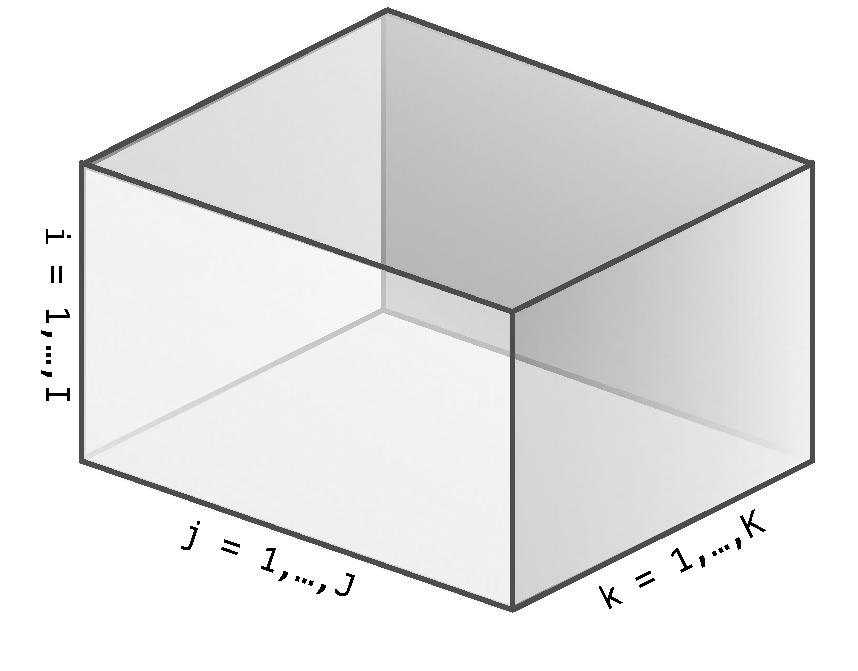
\includegraphics[width=0.4\linewidth]{figs/3dtensor}
  \caption{Example of a 3d tensor.}
  \label{fig:3dtensor}
\end{figure}

A tensor can be interpreted as a multi-way array, as illustrated graphically in \reffig{fig:3dtensor}. This is a 3rd-order tensor. 
We represent tensors by bold underlined capital letter, e.g., $\T{X} \in \R^{I \times J \times K}$. 
The \emph{order} of a tensor is the number of its dimensions or modes, which in the example is 3.
Matrices and vectors are special cases of tensors.
Matrices are 2nd-order tensors, and we denote them by boldface capital letters, e.g., $\M{A} \in \R^{I \times J}$.
Vectors are 1st-order tensors, and we denote them by boldface lowercase letters, e.g., \V{x}.
The elements of a tensor are scalars, and we denote them by lowercase letters, such as $x_{ijk}$ for the $(i,j,k)$ element of a 3rd-order tensor \T{X}.

Given a tensor, we can also ask for a variety of \emph{sub-tensors}.
One form of sub-tensor is a \emph{slice}, which is a 2-dimensional cross-section of a tensor.
\RefFigure{fig:tensor-example}(a) illustrates the concept of slices, showing different slices of a 3rd-order tensor.
Another form of sub-tensor is a \emph{fiber}, illustrated in \reffig{fig:tensor-example}(b).
A fiber is a vector extracted from the tensor, and is defined by fixing every index by one~\cite{Kolda:2009}.

Since slices are all matrices, they can for the 3rd-order example of \reffig{fig:tensor-example}(a) be represented by $\M{X}_{i::}$, $\M{X}_{:j:}$, and $\M{X}_{::k}$.
%For instance, the columns of the matrix $\mathbf{A}=[\mathbf{a_1}, \mathbf{a_2}, \dots, \mathbf{a_J}] \in \R^{I \times J}$ are denoted by $\mathbf{a_j}$. 
In this paper, we consider double-precision real-valued elements for all tensors, matrices, and scalars.

\RefFigure{fig:tensor-example}(b) gives three fibers of the tensor, denoted by $\V{x}_{:jk}, \V{x}_{i:k}, \V{x}_{ij:}$.

\begin{figure}[htbp]
    \centering
    \begin{tabular}{>{\centering\arraybackslash}p{0.45\textwidth}}
%    \includegraphics[scale=0.15]{figs/tensor-example} \\
%    (a) A third-order tensor $\T{X} \in \R^{I \times J \times K}$ (TODO: redo) \\\\
    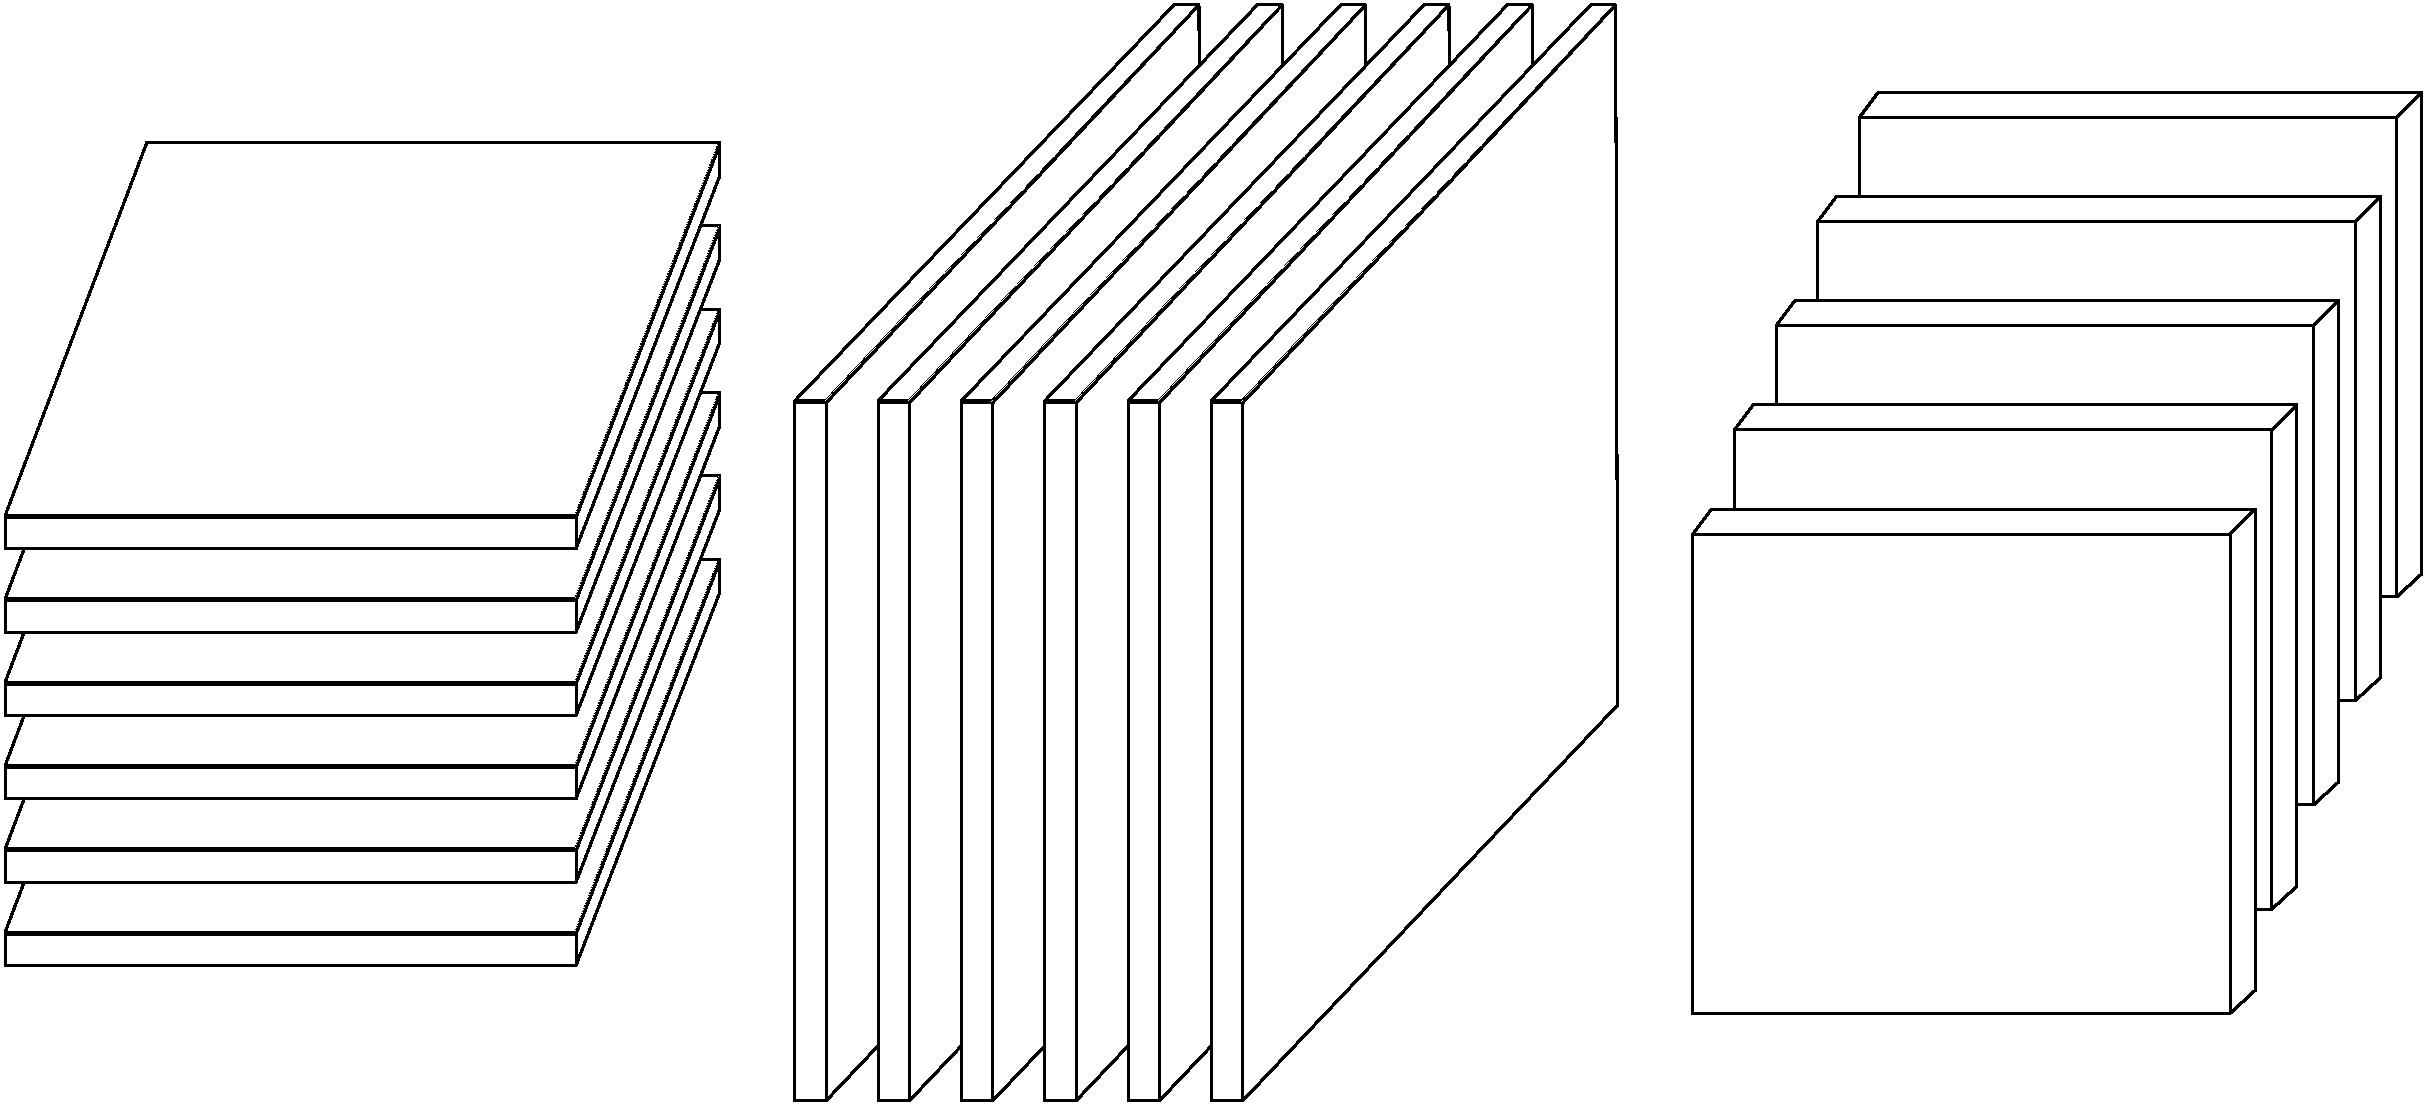
\includegraphics[width=0.55\linewidth]{figs/slices_own} \\
    (a) Horizontal, lateral and frontal slices of a third order tensor \\\\
    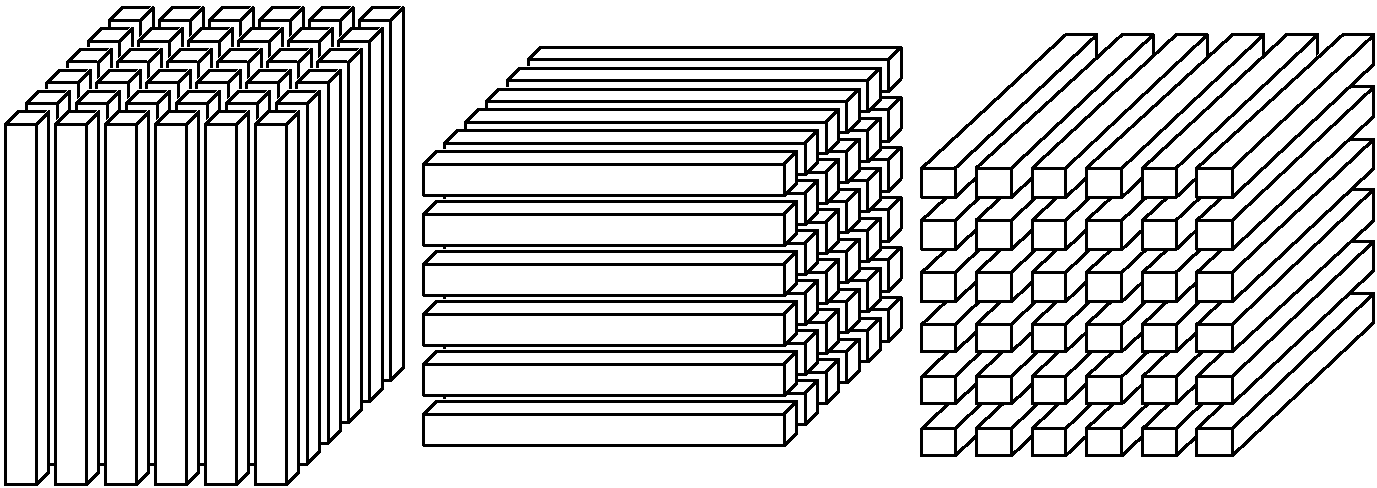
\includegraphics[scale=0.2]{figs/fibers_own} \\
    (b) Column (mode-1), row (mode- 2), and tube (mode-3) fibers of a third order tensor. \\
    \end{tabular}
    \caption{Some sub-tensor views of the third-order tensor $\T{X} \in \R^{I \times J \times K}$.}
    \label{fig:tensor-example}
\end{figure}

Examples of tensor operations include the mode-$n$ product introduced in \refsec{sec:intro}, tensor contraction, and Kronecker product~\cite{Kolda:2009}.
Since the mode-$n$ product is among the most widely used of these primitives, we focus on it in this paper and refer to it alternately as the \acf{Ttm}, following the terminology of the \TensorToolbox~\cite{TensorToolbox}.
%Thus, we focus on mode product as our primary example of tensor multiplications in this paper.
Comprehensive surveys of other tensor operations appear elsewhere~\cite{Kolda:2009, DBLP:journals/corr/Cichocki14}.

The \TTM between a tensor $\T{X} \in \R^{I_1 \times I_2 \times \cdots \times I_N}$ and a matrix $\M{U} \in \R^{J \times I_n}$ is another tensor $\T{Y} = \T{X} \times_n \M{U}$, where $\T{Y} \in \R^{I_1 \times \dots \times I_{n-1} \times J \times I_{n+1} \times \cdots \times I_N}$.
One way to precisely define \TTM is to express it as the element-wise computation,
\begin{eqnarray}
  y_{i_1 \dots i_{n-1} j i_{n+1} \dots i_N}
    & = & (\T{X} \times_n U)_{i_1 \dots i_{n-1} j i_{n+1} \dots i_N} \nonumber \\
    & = & \sum_{i_n=1}^{I_n} x_{i_1 i_2 \dots i_N} u_{ji_n}.
  \label{eq:moden-ele}
\end{eqnarray}
Note that where the input tensor \T{X} is of length $I_n$ in its \varTh{n} mode, the result \T{Y} is of length $J$ in its \varTh{n} mode.
Typically, $J$ will be much less than $I_n$.


The traditional way to execute a \TTM is through \emph{matricization}, also called \emph{unfolding} or \emph{flattening} in the literature.
That is, \TTM is equivalent to a matrix-matrix multiplication in the form,
%
\begin{equation}\label{eq:moden-mat}
  \T{Y} = \T{X} \times_n U \Leftrightarrow \M{Y}_{(n)} = \M{U} \M{X}_{(n)},
\end{equation}
%
where $\M{Y}_{(n)}$ and $\M{X}_{(n)}$ denote the matricized forms of $\T{Y}$ and $\T{X}$, respectively.
For a mode-$n$ product, matricization logically reorders the elements of an order-$N$ tensor into a matrix by exchanging mode $n$ and the leading mode.
The leading mode is dictated by data layout. If data is located in row-major, the last dimension (mode-$N$) is the leading mode.
For instance, a $3 \times 4 \times 2$ tensor with elements from $1$ to $24$ can be arranged as a $3 \times 8$ matrix, or a $4 \times 6$ matrix, or a $2 \times 12$ matrix.
In the tensor context, \emph{vectorization}, $\V{y} = \makeVec(\T{X})$, refers to converting a tensor into an equivalent vector.
The reverse process of creating a tensor from a matrix or vector is called \emph{tensorization}.

\begin{equation}
\label{eq:moden-matricization}
\begin{split}
\M{X}_{(1)} = \left[
\begin{array}{cccccccc}
1 & 4 & 7 & 10 & 13 & 16 & 19 & 22 \\
2 & 5 & 8 & 11 & 14 & 17 & 20 & 23 \\
3 & 6 & 9 & 12 & 15 & 18 & 21 & 24 
\end{array}
\right],\\
\M{X}_{(2)} = \left[
\begin{array}{cccccc}
1 & 2 & 3 & 13 & 14 & 15 \\
4 & 5 & 6 & 16 & 17 & 18 \\
7 & 8 & 9 & 19 & 20 & 21 \\
10 & 11 & 12 & 22 & 23 & 24 
\end{array}
\right],\\
\M{X}_{(3)} = \left[
\begin{array}{ccccccc}
1 & 2 & 3 & \dots & 10 & 11 & 12 \\
13 & 14 & 15 & \dots & 22 & 23 & 24
\end{array}
\right].
\end{split}
\end{equation}

\subsubsection{Multilinear Rank}
Computing rank is NP complete~\cite{HastadRanknp}, and best-rank approximation is ill-posed~\cite{Kolda:2009}
\subsubsection{Tensor Algebra}

\subsubsection{Tensor Contractions}

\subsubsection{Tensor Network Diagrams}
\begin{figure}
  \centering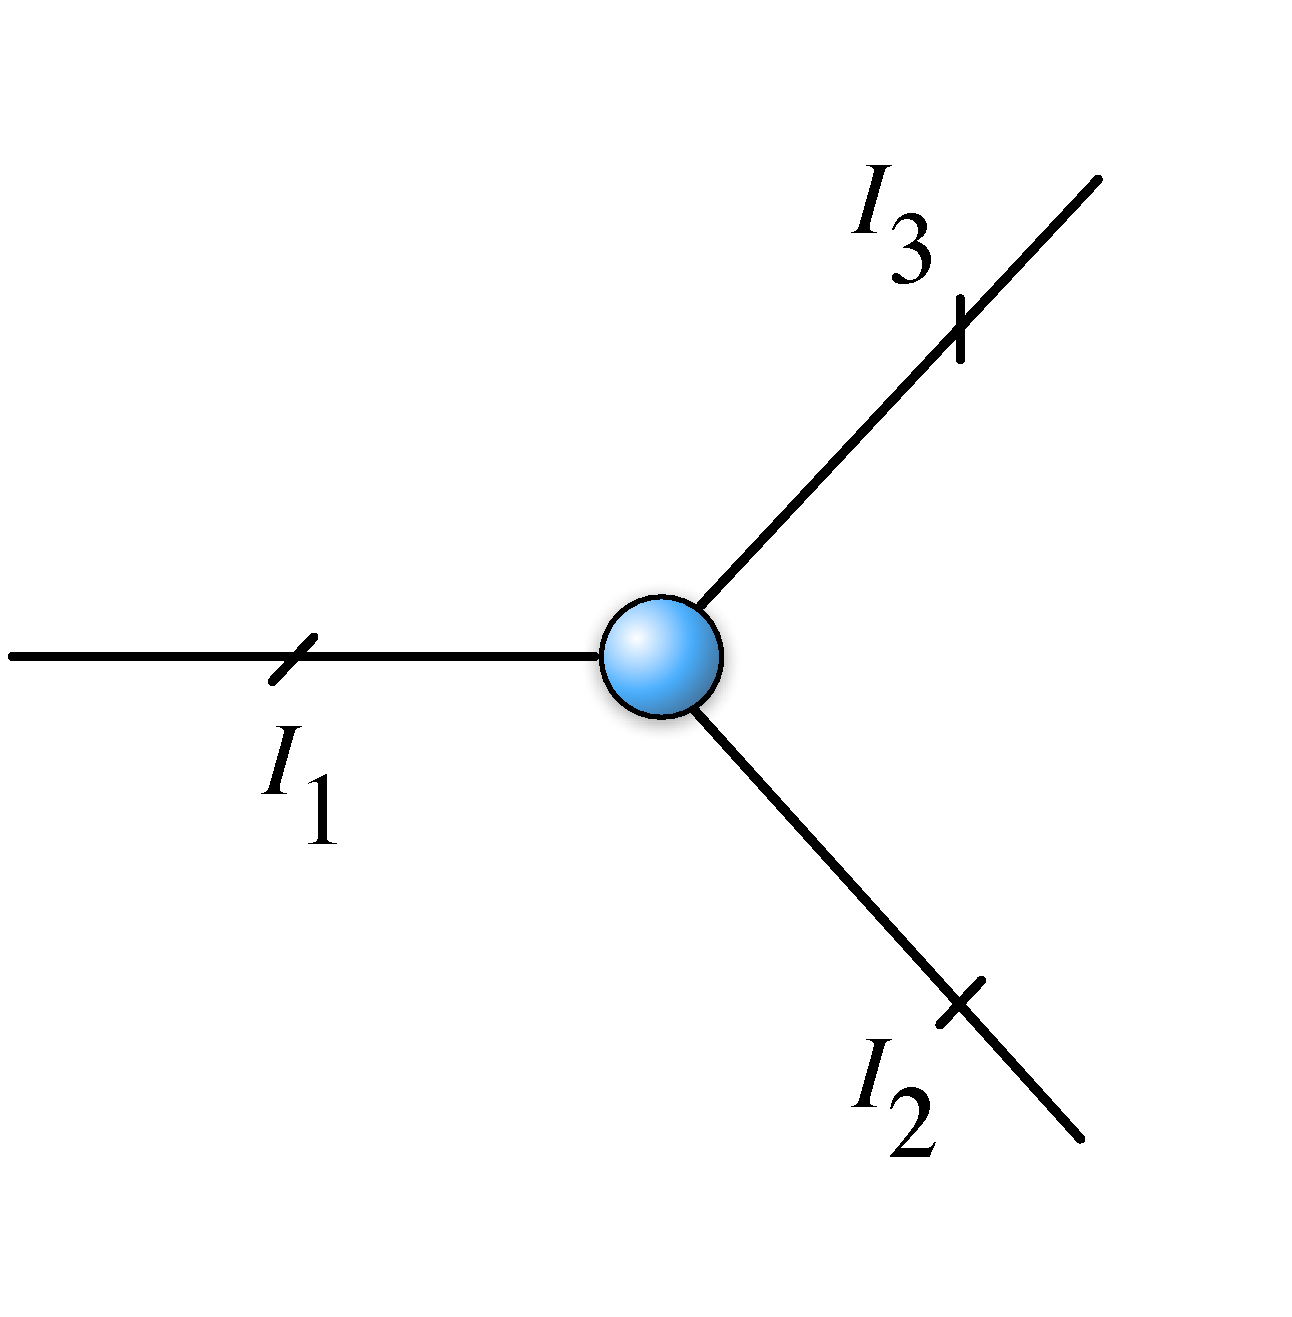
\includegraphics[width=0.3\linewidth]{figs/3dtensornet}
  \caption{Example of 3d tensor representation as a tensor network.}
  \label{fig:3dtensornet}
\end{figure}
% eof

%=======================================================================
\section{Data Science Applications} \label{sec:applications}
                                    In signal processing we may have both temporal and spatial components to our signal (in combination with frequency)

Importance of multi-linear rank-reduction.

Feature selection, feature extraction, classification, multi-way clustering.
Blind-source separation. 
psycho-metrics, chemometrics, signal processing, numerical linear algebra, computer vision, watermarking, numerical analysis, data mining, neuroscience, graph analysis, ICA.
quantum chemistry(Hartree-Fock, MD), EM wave scattering/logging. 3-dimensional PDEs. 

Anandkumar papers~\cite{Anandk}

%eof

%=======================================================================
\section{Low-Rank Approximations}   \label{sec:lowrank}
                                    %mention need for compression
\subsubsection{Tensor Network Diagrams}
\begin{figure}
  \centering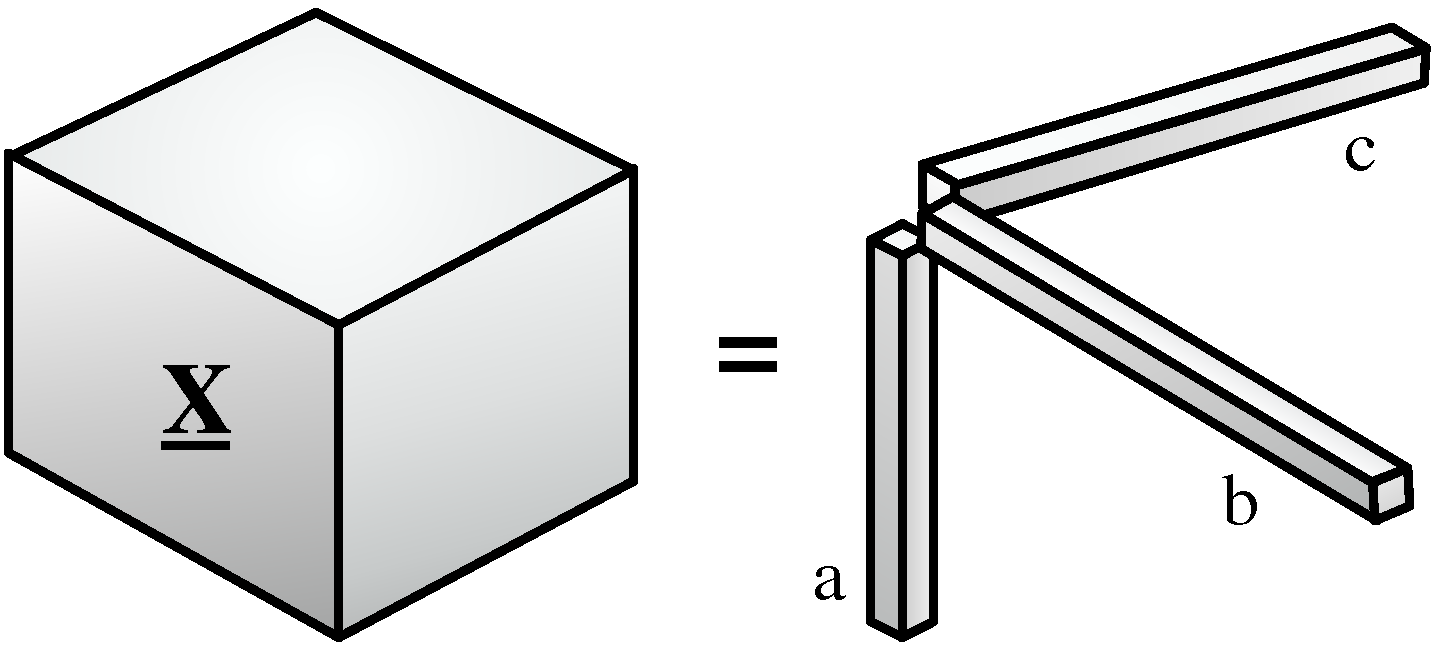
\includegraphics[width=0.5\linewidth]{figs/cpdecomp}
  \caption{CP Decomposition.}
  \label{fig:cpdecomp}
\end{figure}

\subsubsection{Tensor Network Diagrams}
\begin{figure}
  \centering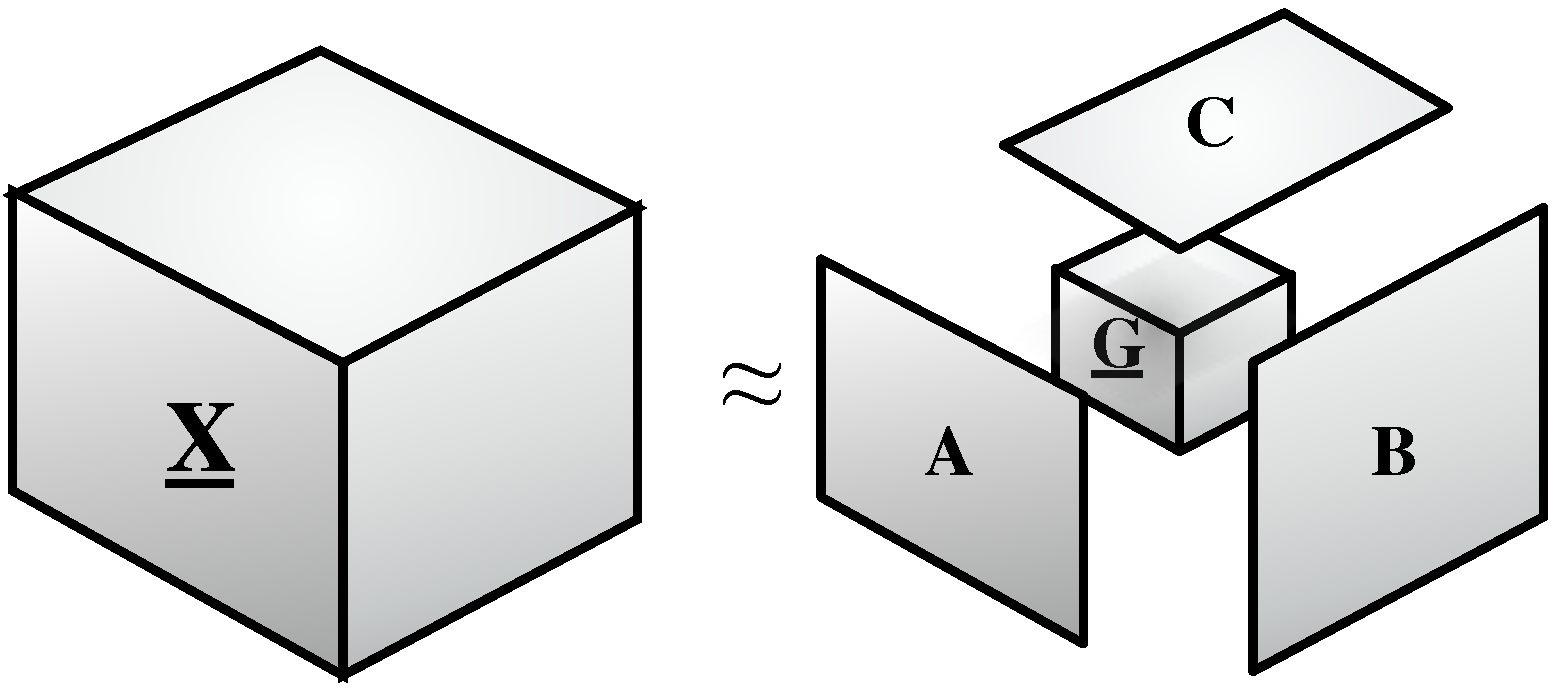
\includegraphics[width=0.55\linewidth]{figs/tdecomp}
  \caption{Tucker decomposition.}
  \label{fig:tdecomp}
\end{figure}

Tucker, CP are old concepts. Decomposition into block terms~\cite{Lathauwer08decompositionsof} generalizes standard methods.

Neat application: Bilinear maps can be generalized as tensors, so tensor decompositions can yield faster algorithms for matrix multiplication, i.e~\cite{Benson}

\subsection{CP Decomposition}
Introduced:~\cite{hitchcock-sum-1927}
CP breaks curse of dimensionality: instead of $n^d$ parameters we need only $dnr$.
CP is ill-posed, different regularizations can be used.
CP assumes every tensor mode is involved with every `concept.' Restrictive for noisy higher order data (-Joachim)
\subsection{Tucker Decomposition}
Introduced:~\cite{Tuck1966c}
Instead of $n^d$ parameters we need only $\prod_{i=1}^d r_i + n\sum_{i=1}^d r_i$.
Stable, we can use SVD~\cite{Lathauwer00amultilinear} To compute using `Tucker HOOI' algorithm~\cite{Lathauwer-THOOI}.
We can determine $r_1, \dots, r_d$ as a function of $\epsilon$.

If the Tucker Decomposition is properly normalized, it is also considered an HOSVD.

Exponential storage, time. In sparse case, we have same problem: dense results (-Joachim)
\subsection{Hierarchical Tucker}
Introduced:~\cite{Grasedyck:2010:HSV:1958286.1958311}
B's can express a linear combination of vectors in the U's below them.
Obst 1: SVD of tensor unfoldings
Obst 2: Intermediate memory blowup (computing core tensor)... dense intermediate result

Tree-adaptive algorithm using clustering~\cite{treeadap}

\subsubsection{Sparse H-Tucker}
If we use CUR decomposition instead of SVD and store only those columns and rows that contain an element, we can greatly reduce storage and retain sparsity of 

\subsection{Tensor Train}
Introduced:~\cite{Oseledets:2011:TD:2079141.2079149}
%=======================================================================

%eof

%=======================================================================
\section{Computational Challenges}  \label{sec:challenges}
                                    \subsection{NP-Hardness}
Most tensor problems, including rank~\cite{HastadRanknp} are NP-Hard~\cite{Hillar}.

\subsection{Curse of Dimensionality}
Does \textsc{ParCube} help here?~\cite{PARCUBE}.

\subsubsection{Time}

\subsubsection{Memory Blowup}
Memory-blowup problem identified and addressed in~\cite{Kolda08scalabletensor}.

In CP-ALS, we have to compute $C\odot B, C\odot A, B\odot A$. Alleviation described in~\cite{Bader07efficientmatlab}

\subsubsection{Storage}

\subsection{Memory Efficiency}

\subsubsection{Representation Issues}
Tensor representations are cache-unfriendly because we may have to load them along any mode.
There are a few proposed solutions~\cite{6408676}

\subsubsection{Distributed Memory Issues}
Mention GigaTensor~\cite{Kang:2012}, which scales much larger than MATLAB but suffers in performance due to MapReduce. 

Discuss DFacTo~\cite{NIPS2014_5395}, another parallel approach. 

Also \textsc{ParCube}~\cite{PARCUBE}


\subsubsection{Communication Bounds}
Recently established by Solomonik, et. al~\cite{commlow}.

\subsection{Computational Scalability}
There is a discussion of recent developments in distributed scalability of tensor algorithms~\cite{falbull}.

\subsection{Sparsity}
SPLATT takes a hyper-graph partitioning approach to reordering based on sparsity pattern~\cite{SPLATT}

\subsection{Stability}
%=======================================================================
%Section on: common operations? computational bottlenecks?

%eof

%=======================================================================
\section{Experiments}               \label{sec:experiments}
                                    \subsection{Breaking Points}

\subsubsection{CP Decomposition}

\subsubsection{Tucker/HOSVD}

\subsubsection{Hierarchical Tucker}

\subsubsection{Tensor Train}

\subsection{Comparisons}

%eof

%=======================================================================
\section{Implementations}           \label{sec:implementations}
                                    The landscape of tensor libraries is growing quickly, but the capabilities of each implementation varies widely and often focuses on a small subset of mathematical methods, often in support of a field-specific application. Native support of tensor data structures is still lacking in nearly every widely-adopted programming language, although powerful open-source libraries are available to the C++ and MATLAB communities. 

While software landscape is expected to change greatly in the near future, this section aims to document the capabilities of current implementations at  publication date.

\subsection{Data Structures}
Recent work has introduced more efficient data structures for distributed dense and sparsetensors.

Discuss Baskaran et. al's representation~\cite{6408676}.

Discuss Cyclops approach~\cite{CTF}.

\subsection{Basic Arithmetic}
(Addition, multiplication)

Discuss indexing approach.

FTensor, LTensor, Blitz++, HUJI

\subsection{Matricization and Tensorization}

\subsection{Tensor Multiplication}

\subsection{Tensor Contraction}
Discuss optimization approaches taken by Tensor Contraction Engine~\cite{TCE} and Cyclops~\cite{CTF,Solomonik:EECS-2014-170}.

Another paper to read from SC14:~\cite{Rajbhandari:2014:CFC:2683593.2683635}

Discuss tensor contraction as the process of computing on a Tensor Network.

\subsection{Tensor Decompositions}
Discuss how a variety of different algorithms can be taken to compute the same decomposition, (i.e ALS, CG, etc) with examples.

Discuss GigaTensor, DFacto.

\subsection{Tensor Networks}
Mention Cichocki survey and a couple of his most interesting results elsewhere. Mention the physics survey~\cite{physnet}


\begin{landscape}
\begin{center}\scriptsize
    \begin{tabular}{ |l  l  c  c  c  c  c  c  c  c  c|}
    \toprule
    \textbf{Implementation} & \textbf{Environment} & $\underline{A} \otimes \underline{B}$ & $\underline{A} \times_n^m \underline{B}$ & \textbf{CP} & \textbf{Tucker} & \textbf{TN} & \textbf{Domain} & \textbf{Dense} & \textbf{Sparse} & \textbf{Distributed} \\ \hline
    \textbf{Tensor Arithmetic} \\
    \hline
    FTensor~\cite{Landry:2003:IHP:1240120.1240122,FTensor}                  
    & C++ & \yesy & \yesy & \non & \non & \non & Phys. & \yesy & \non & \non \\ \myhline
    LTensor~\cite{LTensor}      
    & C++ & \yesy & \yesy & \non & \non & \non & Phys. & \yesy & \non & \non \\ \myhline
    Blitz++~\cite{blitz} 
    & C++ & \yesy & \yesy & \non & \non & \non & Gen. & \yesy & \yesy ? & \non \\ \myhline
    Boost MDA~\cite{boost-multiarray} 
    & C++ & \non & \non & \non & \non & \non & Gen. & \yesy & \non & \non \\ \hline
    \textbf{Tensor Algebra} \\
    \hline
    PyTensor~\cite{Yoo10pytensor:a}             
    & Python & \yesy & \non & \non & \yesy & \non & Gen. & \yesy & \yesy & \non \\ \myhline
    tensor (Theano)             
    & Python & \yesy & \yesy & \non & \non & \non & ML & \yesy & \non & \non \\ \myhline
    C++ Tensor TB           
    & C++ & \yesy & \yesy & \yesy & \non & \non & Gen. & \yesy & \yesy & \non \\ \myhline
    HUJI~\cite{huji}        
    & C++ & \non & \non & \non & \non & \non & Gen. & \yesy & \yesy & \non \\ \myhline
    TCE~\cite{TCE}
    & DSL & \yesy & \yesy & \non & \non & \non & Chem. & \yesy & \non ? & \yesy \\ \hline
    \textbf{Tensor Decompositions} \\
    \hline
    TensorCalculus~\cite{Calculus}
    & C++ & \yesy & \yesy & \yesy & \yesy & \yesy & Gen. & \yesy & \non & \non ? \\ \myhline
    TNT Library~\cite{TNT}
    & C++ & \non ? & \yesy & \non & \non & \yesy & Phys. & \yesy & \yesy & \non \\ \myhline
    Tensor Toolbox~\cite{TensorToolbox}
    & MATLAB & \yesy & \yesy & \yesy & \yesy & \non & Gen. & \yesy & \yesy & \non \\ \myhline
    N-way Toolbox~\cite{Nway-Paper,Nway}
    & MATLAB & \yesy & \yesy & \yesy & \yesy & \non & Chem. & \yesy & \yesy & \non \\ \myhline
    CuBatch~\cite{CuBatch}
    & MATLAB & \yesy & \yesy & \yesy & \yesy & \non & ML & \yesy & \yesy & \non \\ \myhline
    PLS-Toolbox~\cite{PLS-toolbox}
    & MATLAB & \yesy & \yesy & \non & \yesy & \non & Chem. & \yesy & \yesy & \non \\ \myhline
    TDALAB~\cite{TDALAB,TDALAB_online}
    & MATLAB & \yesy & \yesy & \yesy & \yesy & \non & Gen. & \yesy & \yesy & \non \\ \myhline
    TENSORBOX~\cite{TENSORBOX}
    & MATLAB & \yesy & \yesy & \yesy & \yesy & \non & Gen. & \yesy & \yesy & \non \\ \myhline
    Tensorlab~\cite{Tensorlab}
    & MATLAB & \yesy & \yesy & \yesy & \non & \non & Gen. & \yesy & \yesy & \non \\ \myhline
    TT-Toolbox~\cite{tt-toolbox}
    & MATLAB & \yesy & \yesy & \non & \non & \ccell{gray}{TT} & Gen. & \yesy & \non & \non \\ \myhline
    htucker~\cite{HT,Kressner:2014:A9H:2610268.2538688} & MATLAB & \yesy & \yesy & \non & \non & \ccell{gray}{HT} & General & \yesy & \yesy? & \non \\ \myhline
    \hline
    \textbf{Research Implementations} \\
    \hline
    SPLATT~\cite{SPLATT}
    & C & \yesy & \non & \non & \non & \non & Gen. & \non & \yesy & \non \\ \myhline
    GigaTensor~\cite{Kang:2012}
    & C++ & \yesy & \non & \yesy & \non & \non & Gen. & \yesy & \yesy & \yesy \\ \myhline
    DFacTo~\cite{NIPS2014_5395}
    & C++ & \yesy & \non & \yesy & \non & \non & Gen. & \non & \yesy & \yesy \\ \myhline
    Cyclops~\cite{CTF}
    & C++ & \yesy & \yesy & \non & \non & \non & Gen. & \yesy & \non & \yesy \\ \myhline
    \textsc{ParCube}~\cite{PARCUBE}
    & MATLAB & \yesy & \yesy & \yesy & \non & \non & Gen. & \yesy & \yesy & \non \\ \hline
    %scikit-tensor					
    %& Python & \yesy & \yesy & \yesy & \yesy & \non & Phys. \\ \myhline
    \end{tabular}
    \captionof{table}{Software support for native tensor arithmetic and decompositions.} \label{tab:typesupport}
\end{center}
\end{landscape}

%=======================================================================
\section{Conclusions}               \label{sec:conclusions}
                                    
%eof

%=======================================================================
\section{Acknowledgments}           \label{sec:acknowledgments}
                                    
%eof

%=======================================================================
\bibliographystyle{abbrv} \bibliography{tensbib}
\clearpage\newpage
\appendix

% eof

%%%%%%%%%%%%%%%%%%%%%%%%%%%%%%%%%%%%%%%%%%%%%%%%%%%%%%%%%%%%%%%%%%%%%%%%
\end{document}
%%%%%%%%%%%%%%%%%%%%%%%%%%%%%%%%%%%%%%%%%%%%%%%%%%%%%%%%%%%%%%%%%%%%%%%%

%eof